\documentclass{article}
\usepackage{graphicx} % Required for inserting images
\usepackage{caption}    % For figure captions
\usepackage{amsmath}

\title{Intro to AI Project 1}
\author{Sahil Sanghvi (sss426/224007570), Dev Patel, Efrain}
\date{February 2025}

\begin{document}

\maketitle

\section{Part 0}
The "main.py" file is used to create the mazes. First, we are creating a gird of zeros that represent the unvisited cells(they are all unvisited at the start). It then starts at a random cell and begins DFS travesal to visit its neighboring cells. We are using the random function to see if the cells are blocked or not, with a 30 percent probability of being blocked and a 70 percent being unblocked, and then repeating on its unvisited neighbors until the entire grid is visited. 


\section{Part 1}
\subsection*{(a)}
\begin{figure}[h]  % 'h' places the image near the text
    \centering
    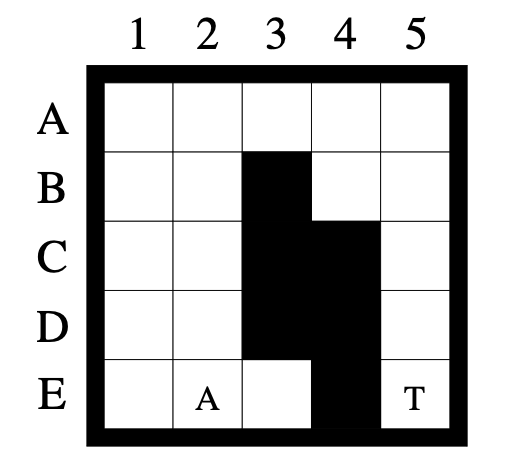
\includegraphics[width=0.5\textwidth]{figure8.png}  % Adjust width as needed
    \caption{Search Problem}
    \label{fig:search_problem}
\end{figure}
In this search problem with the Agent beginning at E2 with the goal at E5, the Agent will initially choose to move east to E3 instead of D2, even if the path between E2 and E5 is blocked. 
This is because of the fact that the Agent makes its decision on where to move based on the f-value of each square, where 
\[f(s) := g(s) + h(s), \]
where \( g(s) \) represents the cost from the start node to the current node, and \( h(s) \) is the heuristic estimate of the cost from the current node to the goal. The heuristic used is the Manhattan Distance and is defined as:
\[h(s) = |x_s - x_{goal}| + |y_s - y_{goal}|\]

where \( (x_s, y_s) \) represents the coordinates of the current state \( s \), and \( (x_{goal}, y_{goal}) \) represents the coordinates of the goal state.

Since the agent does not initially know which cells are blocked, it assumes that all unexplored cells are unblocked and selects the path that minimizes \( f(s) \). In this case, moving east to E3 has a lower \( f(s) \) value than moving north to D2. This happens because:
\[h(E3) = |3-5| + |5-5| = 2,\]
\[h(D2) = |2-5| + |4-5| = 4,\]
\[h(E3) < h(D2) \quad \text{while} \quad g(E3) = g(D2)\]


Therefore, the agent chooses E3 as its first move in the absence of prior knowledge of obstacles. If the agent later discovers that the presumed unblocked path is actually blocked, it will recompute the path and adjust its strategy accordingly.

\subsection*{(b)}

We want to prove that in a finite gridworld, an agent using a search algorithm such as Repeated Forward A* or Adaptive A* will either reach the target or determine that no valid path exists in finite time. Also, we want to prove that the number of moves the agent takes is bounded by the square of the number of unblocked cells.

\subsubsection*{1. The Agent Reaches the Target or Declares It Unreachable}

We assume:
\begin{itemize}
    \item The gridworld has a finite number of cells.
    \item There is a combination of blocked and unblocked cells.
    \item Initially, the agent doesn't know what is blocked and only discovers obstacles as it moves.
    \item The agent follows a search algorithm, such that it explores all reachable unblocked cells.
\end{itemize}

\paragraph{Case 1: The Target is Reachable}
If there exists a valid path from the start to the target:
\begin{itemize}
    \item The search algorithm will eventually find it, as it systematically expands all possible paths.
    \item Since the grid is finite, there are only a limited number of unblocked cells to explore.
    \item The agent expands each unblocked cell at most once and follows the shortest valid path to the target.
\end{itemize}

\paragraph{Case 2: The Target is Unreachable}
If the target is completely surrounded by blocked cells:
\begin{itemize}
    \item The agent will expand all reachable unblocked cells before concluding that the target is inaccessible.
    \item Since there are at most $U$ unblocked cells, the agent will not explore more than $U$ unique positions.
    \item Once all possible paths are exhausted, the agent determines that no valid path exists.
\end{itemize}

Because the grid is finite and the search space is limited, the agent will either reach the target or conclude that it is unreachable in finite time.

\subsubsection*{2. Bounding the Number of Moves by $U^2$}

Let $U$ represent the number of unblocked cells in the grid. A* expands nodes based on the f-value, which is given by:
\[f(s) = g(s) + h(s)\]


In each single execution of A*, the number of expanded nodes is at most $U$, since blocked cells are never expanded.

\paragraph{}
The worst case occurs when the agent explores an incorrect path, encounters an obstacle and must replan, and then repeats this process multiple times until the shortest valid path is found. Since each replanning step involves expanding at most $U$ cells, and the agent may need to replan up to $U$ times in the worst case, the total number of moves is at most:
\[U \times U = U^2\]

\section{Part 2}
When a tie in the f-value of two cells occur, there needs to be a decision about which cell should be expanded first. The smaller g-value strategy expands nodes closer the starting cell, leading to higher runtime and inefficiency, since overall, more paths are explored. In contrast, the larger g-value strategy prioritizes deeper exploration, reducing unnecessary expansions and speeding up the search, as it focuses on searches that get closer and closer towards the goal. Prioritizing smaller g-values creates a strategy that resembles BFS while prioritizing larger g-values is a strategy closer to DFS. Our smaller g-value strategy is about often significantly slower because of this and is usually 10-25 times slower than prioritizing larger g-values.

\section{Part 3}
After comparing both algorithms, we found that their runtime and number of expanded nodes were fairly similar. This is because the entire logic is the same, repeated backwards A* just starts at the goal and ends at the original start. Although the path length remained the same, Repeated Backward A* often performed slightly better, expanding fewer nodes and running faster than Repeated Forward A*. Specifically, it had a 2-7 percent reduction in expanded cells and a quicker overall runtime, however it was not a significant difference.

\section{Part 4}

\subsection{}

A heuristic function $h(s)$ is consistent if the heuristic satisfies:
\[ h(s) \leq c(s, s') + h(s') \]
for every state $s$ and its successor $s'$, where $c(s, s')$ is the cost of moving from $s$ to $s'$. In a gridworld where movement is restricted to the four main directions, the Manhattan distance heuristic is defined as:

   \[h(s) = |x_s - x_g| + |y_s - y_g| \] 

where $(x_s, y_s)$ are the coordinates of current cell $s$, and $(x_g, y_g)$ are the coordinates of the goal $g$.

Consider moving from a cell $s$ to a neighboring cell $s'$. In a four-connected grid, the cost of moving is typically $c(s, s') = 1$. There are two possible cases:

\begin{itemize}
    \item If we move closer to the goal, then one of the absolute differences in the Manhattan distance decreases by 1, while the other remains the same.
    \[ h(s') = (|x_s - x_g| - 1) + |y_s - y_g| \]
    or
    \[ h(s') = |x_s - x_g| + (|y_s - y_g| - 1) \]
    
    Thus,
    \[ h(s) - h(s') = 1 \text{ and } 1 = c(s, s')\]
    which satisfies the consistency condition.
    
    \item If we move in a direction that increases the Manhattan distance, then:
    \[ h(s') = (|x_s - x_g| + 1) + |y_s - y_g| \]
    or
    \[h(s') = |x_s - x_g| + (|y_s - y_g| + 1)\]
    In this case,
    \[h(s) - h(s') = -1 \leq 1 = c(s, s')\]
    which still satisfies consistency.
\end{itemize}

Since this proof holds for all cases where the agent moves towards the goal or away from the goal, we can conclude that the Manhattan distance remains consistent as a heuristic when the agent can only move in the four main directions.

\subsection{}

Adaptive A* updates the heuristic function dynamically as follows:
    \[ h_{\text{new}}(s) = \max(h(s), g^*(s) - g^*(s_{\text{start}})) \]

where:
\begin{itemize}
    \item $h(s)$ is the previous heuristic value.
    \item $g^*(s)$ is the actual optimal cost-to-goal from state $s$.
    \item $g^*(s_{\text{start}})$ is the optimal cost from the start state.
\end{itemize}

A heuristic is admissible if it never overestimates the true cost-to-goal:
    \[h_{\text{new}}(s) \leq g^*(s)\]
$h_{\text{new}}(s)$ is updated using:
    \[h_{\text{new}}(s) = \max(h(s), g^*(s) - g^*(s_{\text{start}}))\]

Since the original heuristic doesn't overestimate the true cost to the goal, it's already admissible. The updated value,  $g^(s) - g^(s_{\text{start}}),$  is always at most  $g^(s)$  because  $g^(s_{\text{start}})$  represents a lower bound on all of the cost to goal values. Therefore,  $h_{\text{new}}(s)$  remains admissible.

\paragraph{}
To show that Adaptive A* maintains consistency, we need to check that for any successor $s'$ of $s$:
    \[h_{\text{new}}(s) \leq c(s, s') + h_{\text{new}}(s')\]

Given that $h_{\text{new}}(s)$ is updated using $\max(h(s), g^*(s) - g^*(s_{\text{start}}))$, we consider two cases:

\begin{itemize}
    \item If $h_{\text{new}}(s) = h(s)$ and $h_{\text{new}}(s') = h(s')$:
    The original heuristic was already consistent as proven previously, so:
    \[h(s) \leq c(s, s') + h(s')\]
    holds, which means consistency is preserved.

    \item If $h_{\text{new}}(s) = g^*(s) - g^*(s_{\text{start}})$:
    The optimal cost-to-goal satisfies:
    \[g^*(s) \leq c(s, s') + g^*(s')\]
    Since $h_{\text{new}}(s') \geq g^*(s') - g^*(s_{\text{start}})$, we get:
    \[g^*(s) - g^*(s_{\text{start}}) \leq c(s, s') + (g^*(s') - g^*(s_{\text{start}}))\]
    which implies:
    \[h_{\text{new}}(s) \leq c(s, s') + h_{\text{new}}(s')\]
\end{itemize}

Thus, Adaptive A* maintains consistency after updating the heuristic.

\paragraph{}
Based on these previous proofs, we have been able to conclude that the Manhattan distance heuristic is consistent in a four-connected gridworld and the fact that Adaptive A* maintains heuristic consistency even when action costs increase.

\section{Part 5}
Both of these algorithms are pretty similar and have almost the same run time. We found that Adaptive A* is slightly faster compare to Repeated Forward A*. In our cases, it was about 2-10 percent faster in terms of average cells expanded. Also, in certain cases where we run an adaptive A* search on the same maze twice with the same start and goal, keeping the $h_{values}$ dictionary between runs we see an improvement in terms of finding a more optimal path and expanding less cells. 

\section{Part 6}
To determine whether the performance differences between two search algorithms are systematic or due to sampling noise, we can use a statistical hypothesis test, such as the paired t-test or the Wilcoxon signed-rank test. We are going to use paired t-test to find any significant differences in Part 3 or 5. For Part 3, the null hypothesis would be that there is no significant difference in the number of expanded nodes between Repeated Forward A* and Repeated Backward A*; any observed difference is due to random variation. The Alternative Hypothesis would states that Repeated Backward A* expands fewer nodes than Repeated Forward A*. Then we would collect the data that supports or opposes this hypothesis, by running these searches on a large number of mazes, making sure each type of search runs on each maze. Then you would compute the test statistic(t-value), and compare it to the p-value. If the t-value is less than 0.05 it would mean that our alternate hypothesis is supported and Repeated Backward A* actually outperforms Repeated Forward A*. On the other hand, if the p-value is greater than or equal to 0.05 then the observed difference is not statistically significant, meaning it could be due to random variation.


\end{document}
